\ignore{
\begin{verbatim}
  * Impact on performance (IPC)
  * Impact on energy
  * Coverage
  * Deep Dive
    * Cache characterization 
        Locality impact?
    * Slice statistics 
        Instruction mix, length, ...
    * Recomputation overhead?
    * Sensitivity analysis?
    * ...
 \end{verbatim}
 }

\ignore{
\begin{figure}[t]
  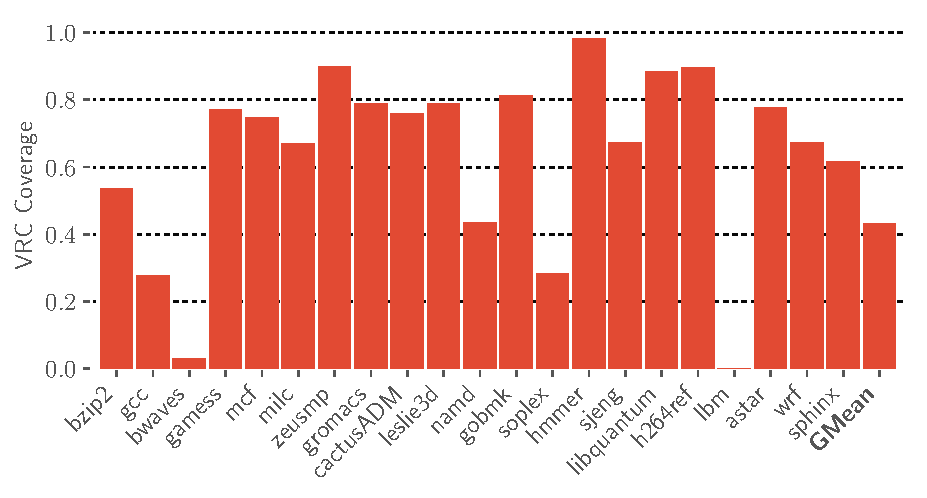
\includegraphics[width=\columnwidth]{figs/vrc_coverage.pdf}
  \caption{The coverage of the \recomp, i.e., the ratio of shadowed L1 misses that can be recomputed instead of being delayed.}
  \label{fig:rc-coverage}
\end{figure}

\begin{figure}[t]
  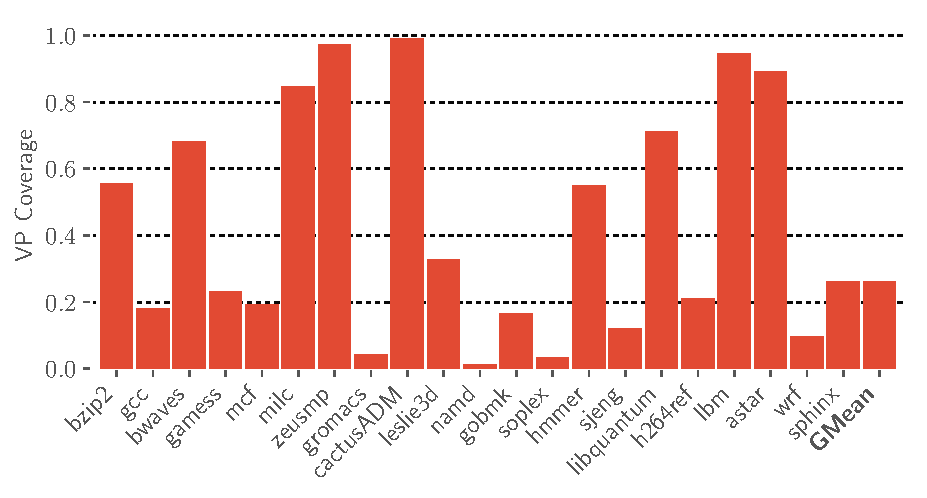
\includegraphics[width=\columnwidth]{figs/vp_coverage.pdf}
  \caption{The coverage of the VP, i.e., the ratio of shadowed L1 misses that can be predicted instead of being delayed.}
  \label{fig:vp-coverage}
\end{figure}
}

\begin{figure}[t]
  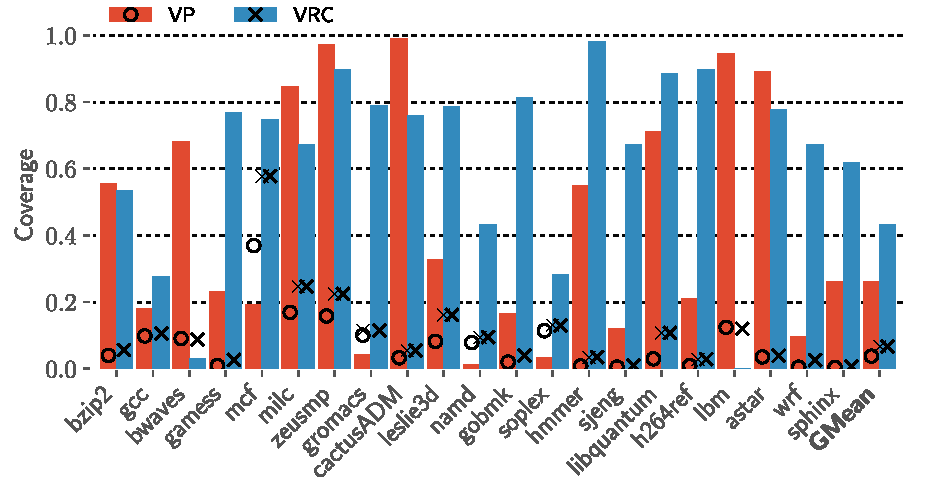
\includegraphics[width=\columnwidth]{figs/coverage.pdf}
  \caption{The coverage of the VP and the \recomp, i.e., the ratio of shadowed L1 misses that can be recomputed instead of being delayed (bars). Also on the same plot, the L1 miss ratio for both versions can be seen (circles/crosses).}
  \label{fig:coverage}
\end{figure}

\begin{figure}[t]
  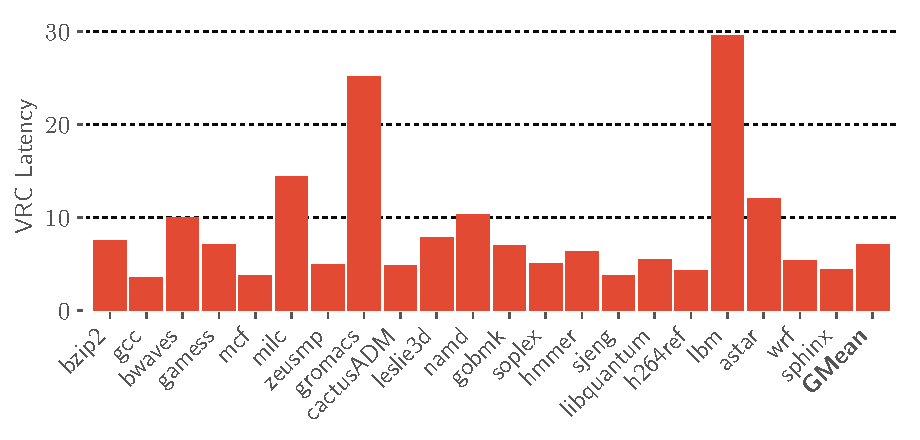
\includegraphics[width=\columnwidth]{figs/vrc_latency.pdf}
  \caption{The mean latency for recomputing a shadowed L1 miss.}
  \label{fig:rc-latency}
\end{figure}

\begin{figure*}[t]
  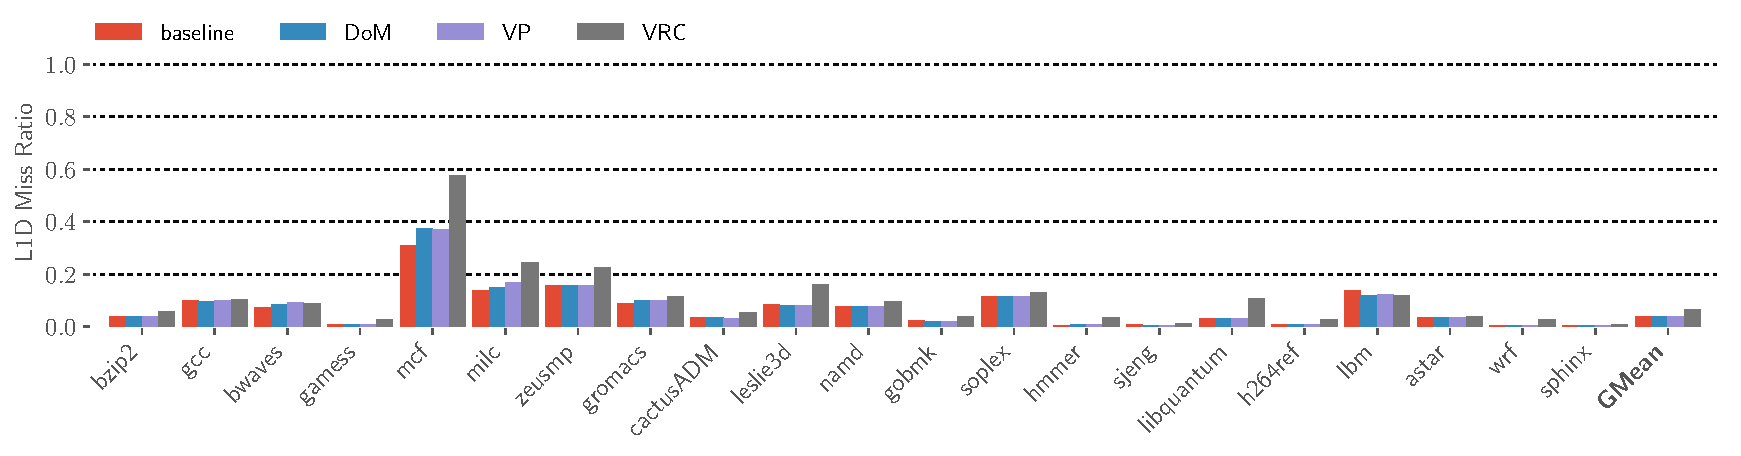
\includegraphics[width=\textwidth]{figs/l1d_miss_ratio.pdf}
  \caption{L1D miss ratio for Delay-on-Miss with VR and \recomp.}
  \label{fig:l1d_misses}
\end{figure*}

\begin{figure*}[t]
  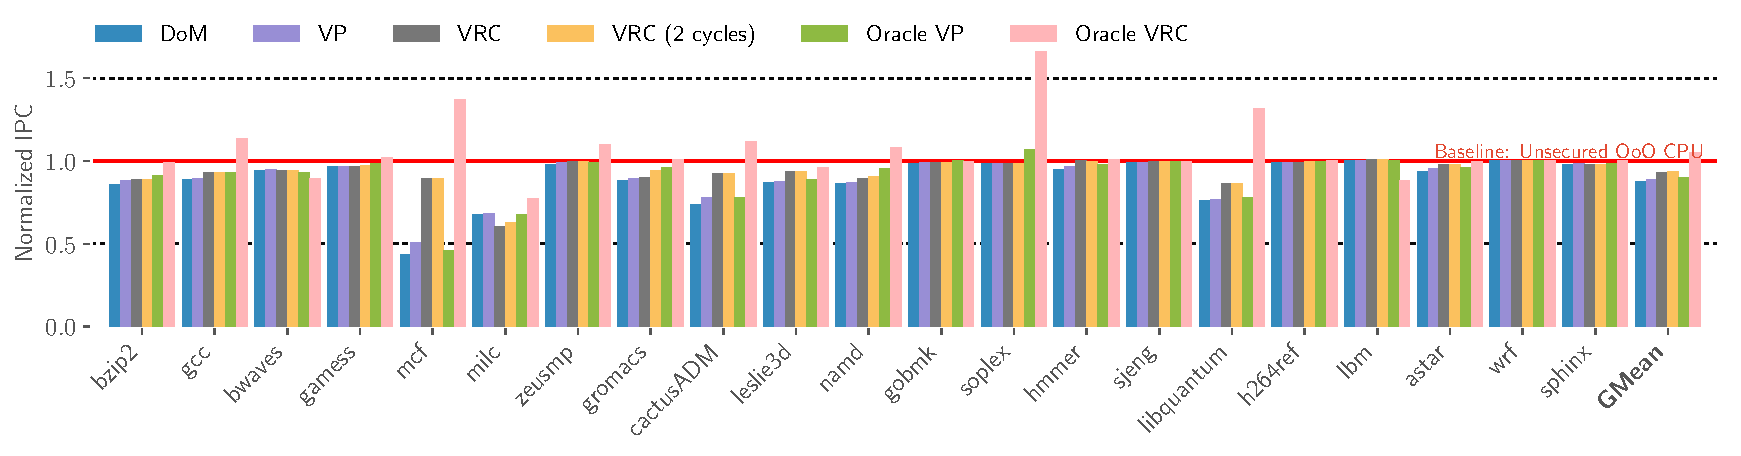
\includegraphics[width=\textwidth]{figs/normalized_ipc_all.pdf}
  \caption{Performance (IPC -- higher is better) normalized to an unsecured OoO baseline.}
  \label{fig:ipc}
\end{figure*}


\begin{figure*}[t]
  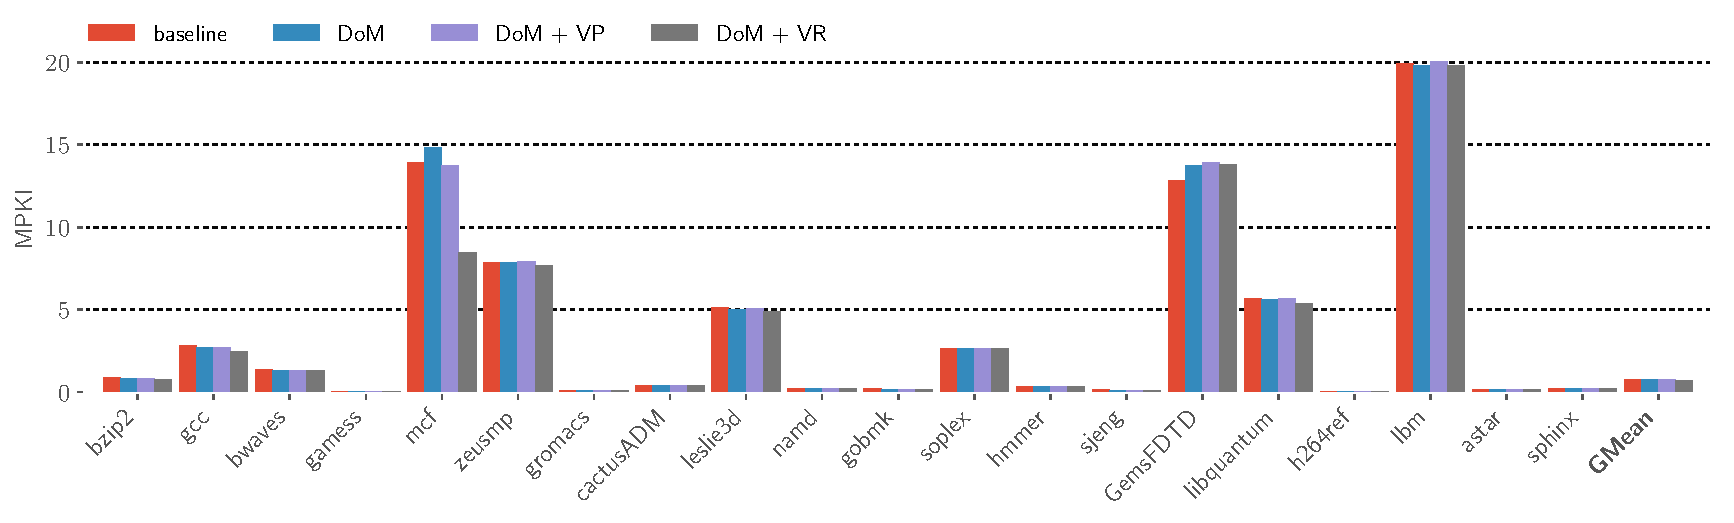
\includegraphics[width=\textwidth]{figs/mpki.pdf}
  \caption{LLC misses per 1000 instructions (MPKI).}
  \label{fig:mpki}
\end{figure*}

\begin{figure*}[t]
  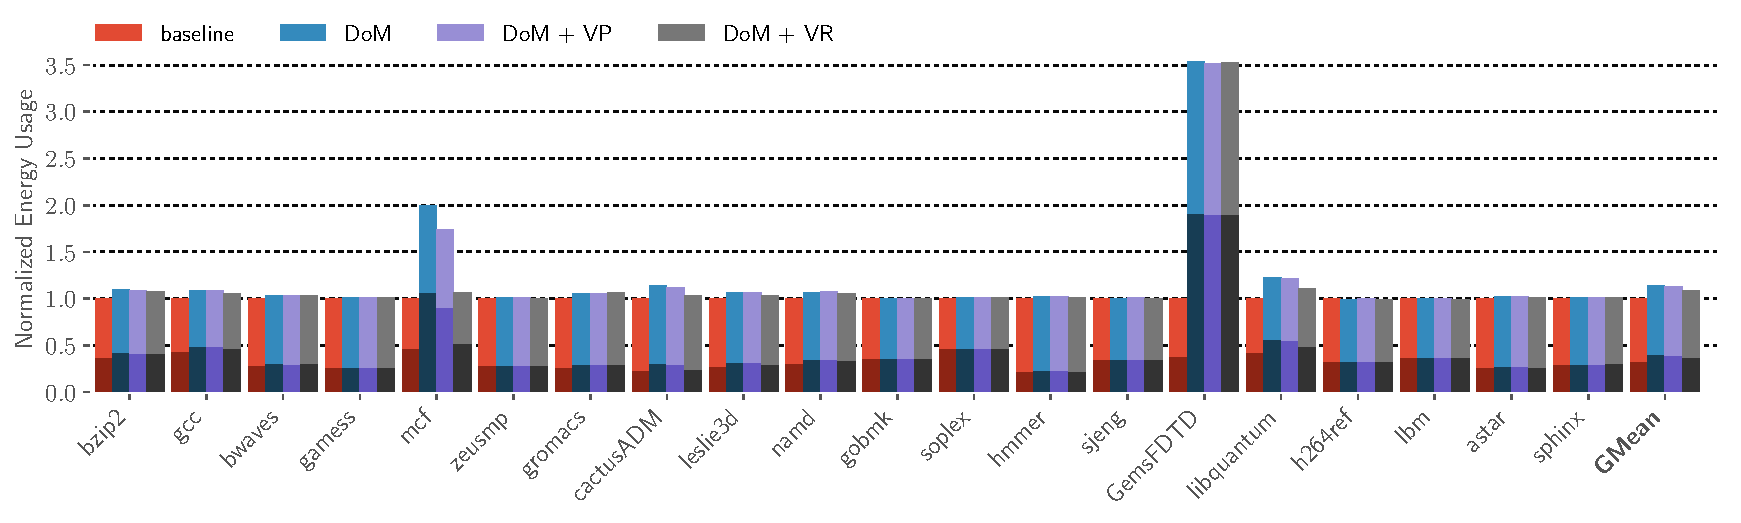
\includegraphics[width=\textwidth]{figs/normalized_energy_usage.pdf}
  \caption{Energy usage, where each bar consists of four parts (from bottom up): The bottom, light colored part is the dynamic energy of the CPU, the middle, dark colored one is the static energy of the CPU, the middle light part is the DRAM energy, including refresh and power-down energy, and the top dark part is the overhead of VP and VRC, both static and dynamic.
  }
  \label{fig:energy}
\end{figure*}

%\redHL{We should have a couple of lines of text here, between the section header and the subsection.}

\subsection{Recomputation Coverage}
\label{sec:coverage}

The coverage for the {\recomp} can be seen in \autoref{fig:coverage}, together with the VP coverage. We can immediately observe that, on average, VRC has higher coverage than VP, at $43\%$ of all speculative L1 misses vs $26\%$ with the VP. A notable example is \texttt{mcf}, which is one of the worst performing benchmarks with DoM (\autoref{sec:performance}). On the other hand, \texttt{lbm} is a counter-example, where we have almost zero VRC coverage. This, however, does not affect the performance negatively, as \texttt{lbm} does not suffer from any performance penalties even with the plain DoM.

On the same figure we have also superimposed the cache miss ratio for both versions. We only predict or recompute L1 misses, so the miss ratio is needed in conjunction with the coverage to infer the percentage of loads in the application that are being predicted or recomputed. More detailed L1D miss data can be found in \autoref{fig:l1d_misses}. Note how, as discussed in~\autoref{sec:limitations}, \recomp{} increases the miss ratio.

With VP, all loads that can be predicted are predicted in the same amount of time (2 cycles in our setup), but the same is not true for the VRC, where the latency depends on the slice length and the instructions it contains. In \autoref{fig:rc-latency} we can see the mean recomputation latency for each benchmark, as well as the overall mean. In all cases, VRC requires more cycles than VP to recompute a value, with a mean of seven cycles per slice. However, as we will see in~\autoref{sec:performance}, this does not impact the performance significantly.

\subsection{Performance}
\label{sec:performance}

\autoref{fig:ipc} contains the number of committed instructions per cycle, normalized to the unsecured baseline processor. 
Delay-on-Miss without VP or \recomp, which is our \emph{secure} baseline, performs at $88\%$ of the unsecured baseline, similarly to the results reported by Sakalis et al~\cite{sakalis+:ISCA2019vp}. 
%The two benchmarks that incur the biggest hit in performance are \texttt{GemsFDTD} (at $20\%$ of the baseline) and \texttt{mcf} ($44\%$), followed by \texttt{cactusADM} ($74\%$) and \texttt{libquantum} ($76\%$). 
The benchmarks that incurs the biggest hit in performance is \texttt{mcf} (at $44\%$ of the baseline), followed by \texttt{milc} ($68\%$), \texttt{cactusADM} ($74\%$) and \texttt{libquantum} ($76\%$).
Out of these benchmarks, three (\texttt{mcf}, \texttt{milc}, and \texttt{libquantum}) have high LLC MPKI (\autoref{fig:mpki}), but that in itself is not the only factor, as other benchmarks (e.g., \texttt{lbm}) also have a high MPKI. 
Instead, the cost of Delay-on-Miss also depends on the amount of MLP that the benchmarks exhibit; the more MLP that is taken advantage of in the baseline, the higher the performance loss. 
%This is particularly true for \texttt{GemsFDTD}, which is one of the benchmarks with a large number of concurrent long latency loads to multiple cache lines.

If VP is introduced, then the performance is similar, at $89\%$ of the unsecured baseline.
This result contradicts the results given by Sakalis et al.~\cite{sakalis+:ISCA2019vp}, where the VP gives a significant performance advantage\footnote{We contacted the authors and verified that our results are indeed valid.}. %TODO: This should be rewritten when we are no longer anonymous
The reason that VP does not offer a significant advantage is because VP itself is speculative: When a value is predicted it still needs to be validated at a later point. 
By predicting the value, a small amount of parallelism (ILP) can be exploited during execution, but the slow L1 misses still need to be satisfied for the validation. 
Due to the high number of speculative shadows, validations becomes serialized and are not able to take advantage of any MLP that might be found in the application. 
In essence, the VP pushes the cost of delaying speculative loads from the execution stage to the validation stage, but it does not eliminate it. 
This can be seen in the Oracle VP results, where even $100\%$ prediction rate (i.e., all shadowed L1 misses are successfully predicted) only leads to a marginal performance improvement of one percentage point.

The same is not true for \recomp, as once a value has been recomputed, it does not need to be validated, meaning that the cost for delaying a long latency miss is eliminated and no  serialization is enforced.
While \recomp{} does not increase the amount of MLP that can be taken advantage of, it does eliminate some of the need for it.
Overall, \recomp{} performs at $93\%$ of the unsecured baseline, decreasing the performance cost of Delay-on-Miss by more than one third (specifically, by $42\%$).
The benchmark with the most dramatic performance increase is \texttt{mcf}, which is the worst performing benchmark for Delay-on-Miss. 
\recomp{} improves the performance from $44\%$ to $90\%$, reducing the performance cost to one fifth of that of Delay-on-Miss. 
%\redHL{Unfortunately, in the case of \texttt{GemsFDTD} (the worst performing benchmark), we have a very low slice coverage, meaning that most of the loads cannot be recomputed.} 
%Because of this, \recomp, much like VP, does not improve the performance over Delay-on-Miss.

We have also evaluated an artificial version of \recomp{} where we keep the same slice coverage but reduce the cost of the slices to at most two cycles. This version exhibits almost identical performance to the real \recomp{}, with a mean performance difference of half a percentage point. This strongly indicates that instead of trying to keep the cost of the slices low, it is more important to increase the coverage, even if large slices are required. This is further corroborated by the results from the Oracle version, discussed below. However, large slices do increase the energy usage, as we will see in ~\autoref{sec:energy}, so a balance still needs to be kept.

If we introduce an Oracle \recomp{} that can recompute all shadowed L1 misses, the difference between the VP and the \recomp{} approaches becomes even more apparent. 
Both Oracle versions have $100\%$ coverage and the same latency, the only difference is that with VP the loads need to be validated when they are unshadowed, while with \recomp{} they are completed as soon as the value has been recomputed.
While, as we have seen, the VP Oracle can only achieve marginal improvements over the non-Oracle version, the \recomp{} Oracle is able to outperform even the baseline, including benchmarks such as \texttt{mcf}, \texttt{cactusADM}, and \texttt{libquantum}.
Of course, such an Oracle is unrealistic, but it does support our argument that the limiting factor for VP is the cost of validation.
%Additionally, given the $3.5\times$ over the baseline performance improvement we can observe in \texttt{GemsFDTD}, it further validates our analysis that \texttt{GemsFDTD} suffers from a lot of long latency misses that require a lot of MLP to hide.}


However, it is worth noting here that a 100\%-coverage {\recomp} does not necessarily guarantee that the performance will exceed that of the baseline. In fact, there are four benchmarks where the Oracle VRC is slower than the baseline: \texttt{bwaves}, \texttt{milc}, \texttt{leslie3d}, and \texttt{lbm}. Out of these, the \texttt{bwaves} and \texttt{lbm} {\recomp} Oracle is also slower than DoM.
There are various factors that contribute to this result: In \texttt{bwaves} and \texttt{leslie3d} the L1 and the L2 miss ratio (not shown) is increased significantly with the Oracle; in \texttt{milc} the Oracle increases the number of write misses in the L1 (not shown), as well as the average write miss latency (not shown); finally in \texttt{lbm} a combination of many factors contribute to worse cache performance.
The problem is that, even with $100\%$ coverage, not every single memory access is recomputed: Stores, non-speculative loads, and speculative L1 misses that hit in the MSHRs, are still served by the memory hierarchy. By recomputing the rest of the loads, which account for the majority of the L1 misses, the Oracle \recomp{} disrupts the normal operation of the cache and the prefetcher, resulting in performance losses. Essentially, there is a trade-off between the benefits of eliminating long-latency L1 misses and the cost of disrupting the normal cache operation.
For the majority of the benchmarks, this trade-off leans towards the benefits, but this is not true for all of the benchmarks.
Future work aiming to increase {\recomp} coverage must account for these factors to achieve optimal performance.
%I believe that the reason for the performance cost is disrupting the cache. For the paper, I am not 100\% convinced I can explain all of them in detail, so I suggest going with the more generic approach: VRC disrupts the cache, which causes performance loss, and there is a trade-off between this loss and the gain from recomputation.



\subsection{Energy Efficiency}
\label{sec:energy}

Energy efficiency, in our case, is affected by three main factors: The execution time/performance, the number of accesses in the memory hierarchy (especially the DRAM), and the cost of predicting (VP) or recomputing (VRC) a value.
\autoref{fig:energy} shows, starting from the bottom, the dynamic (bottom, light color) and static (middle, dark color) energy of the CPU, the total DRAM energy (middle, light), and, finally, the overhead (if any) for VP and VRC (top, dark). %
Overall Delay-on-Miss and VP increase the mean energy usage over the unsecured baseline by $6\%$, while \recomp{} increases it by $5\%$. The dynamic energy of the CPU (excluding the overheads) remains mostly the same across all versions, instead it is the static, DRAM, and overhead energy that changes.

Static energy is affected because the execution time is affected. This is most obvious in \texttt{mcf}, the application with the worse DoM performance, followed by \texttt{milc}. As can be seen in~\autoref{fig:mpki}, none of the evaluated solutions affect the MPKI significantly, so the increase in the DRAM energy is not due to an increase in the number of accesses but due to other operations such as refresh and power-down states. These operations do depend on the access patterns, but they also depend on the execution time, similar to the static energy usage of the system.

On the other hand, the overheads introduced by the VP and the \recomp{} are affected both by the execution time (static energy) and by the operations performed. This is particularly visible in the case of the \recomp{}, where the majority of the overhead is due to the instructions of the slices. As we have discussed in ~\autoref{sec:performance}, smaller slices do not lead to better performance, but the same is not true for the energy costs. Instead, a balance between coverage (which increases the performance) and slice length (which increases the energy usage) needs to be achieved, but such an exploratory study is beyond the scope of this work and is left as future work.

Out of all the benchmarks, the ones with the highest (relative to the baseline) energy usage are \texttt{milc} (at $37\%$ over the baseline), \texttt{gromacs} ($13\%$) and \texttt{libquantum} ($12\%$). The rest of the benchmarks have energy overheads of less than $10\%$ over the baseline. \texttt{milc} is the benchmark with the worse performance, so part of the energy increase is due to static and DRAM energy. It also has a high \recomp{} coverage and also some of the third most expensive (in cycles, on average) slices among all the benchmarks, which increases the \recomp{} overhead energy. On the other hand, \texttt{gromacs}'s performance comes very close to the baseline, but it does have the second most expensive slices, while also having high coverage. Finally, \texttt{libquantum} also sees an increase in execution time and by extension, energy usage. The next benchmark with the higher energy increase over the baseline is \texttt{mcf} ($9\%$), but this is far better than DoM, with or without VP, which is at $63\%$ and $84\%$ respectively.

%\texttt{GemsFDTD} and \texttt{mcf} incur a $3.5\times$ and $2\times$ performance overhead respectively. 
%As previously discussed in the performance analysis (\autoref{sec:performance}), \recomp{} does not improve the results for \texttt{GemsFDTD} due to low coverage, but it does decrease the overhead for \texttt{mcf} to just $6\%$ over the baseline. 
%This is a combination of both reducing the execution time and reducing the MPKI/DRAM accesses. 
%In contrast, the VP incurs an overhead of $1.7\times$ over the baseline.

%\subsection{Memory Behavior}
%\label{sec:memory}